\subsection{Direkte Evaluation der Erklärungen}
\label{sec:study_results_qualitativ}

Die zuvor analysierten Metriken betreffen ausschließlich die Auswirkungen von Erklärungen auf die \textit{Objectives} für die Integration - im konkreten Fall \textit{Usage Increase}, \textit{System Acceptance} und \textit{Satisfaction}.

Mithilfe der Metriken konnte Überprüft werden, welche Erklärungen, in welchen Kombinationen den zuvor aufgestellten Anforderungen genügen. Da allerdings keine klare Empfehlung abgeleitet werden kann, welche der Erklärungen weiterhin 

Zuvor wurden die Metriken, welche zur Überprüfung 

Da aus den Einflüssen, die durch die Erklärungen auf die Metriken, welche f

\subsubsection{Ziel der direkten Evaluation}

\subsubsection{Methode}

\subsubsection{Ergebnisse}

\subsubsection{Bedarf für die gegebenen Erklärungen}

Die statischen Erklärungen (siehe \autoref{sec:user_count_definition} und \autoref{sec:route_explanation_definition}), welche die Einflüsse auf den Routing-Algorithmus von NUNAV sowie das kollaborative Routing erklären, sind interaktiv. Somit kann evaluiert werden, wie viele Studienteilnehmer wie häufig diese angefordert haben. Außerdem kann gemessen werden, wie lange sie die Erklärungen betrachtet haben.

Die drei verschiedenen Erklärungen, die die Nutzer aufrufen können, sind in \autoref{sec:user_count_definition} und \autoref{sec:route_explanation_definition} beschrieben. Die Studiengruppen (Gruppe 2 und 4), denen diese angezeigt wurden enthalten insgesamt 1 766 Teilnehmer.

Im Folgenden wird die Erklärung zum Routing-Algorithmus \textit{Erklärung 1}, die kurze Erklärung zum kollaborativen Routing als \textit{Erklärung 2} und die dazugehörige weitere Erklärung als \textit{Erklärung 3} genannt.

Als gelesen bzw. zumindest entschieden, ob die Erklärung benötigt wird gilt diese, wenn ein Nutzer länger als 1,5 Sekunden in dem Dialog verbracht hat \cite{BAHR2011776}. \autoref{fig:explanation_results_clicked} zeigt wie häufig die Nutzer eine Erklärung angefordert haben und diese auch zumindest zum Teil gelesen haben. \autoref{tab:explanation_results_clicked} zeigt die Bewertung als \glqq Hilfreich\grqq{} oder \glqq Nicht hilfreich\grqq{} durch die Nutzer. Allerdings sind die Hilfe-Artikel auch über andere Wege erreichbar, wodurch Bewertungen nicht nur von Nutzern kommen, die über die NUNAV-App dort hingeleitet wurden.

\begin{figure}[htb!]
    \centering
    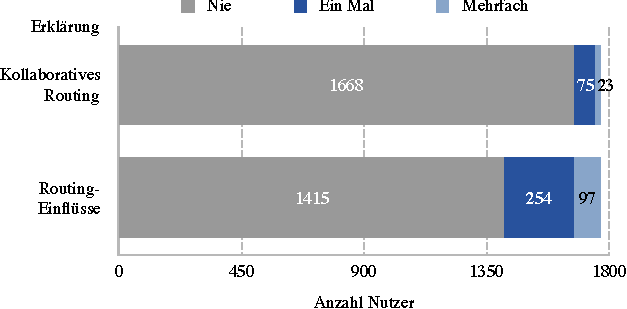
\includegraphics[width=\textwidth]{contents/06_model_evaluation/02_evaluation/res/explanation_results_clicked.pdf}
    \caption{Anzahl der Nutzer, die Erklärungen gelesen haben}
    \label{fig:explanation_results_clicked}
\end{figure}

\begin{table}[htb!]
    \centering
    \begin{tabular}{p{.5\textwidth}p{.15\textwidth}p{.25\textwidth}}
        \hline
        Artikel & Hilfreich & Nicht Hilfreich \\
        \toprule
        Kollaboratives Routing & 76 & 9 \\
        Einflüsse auf die Routenberechnung & 209 & 32 \\
        \bottomrule
    \end{tabular}
    \caption{\textit{Usefulness} der Hilfe-Center-Artikel}
    \label{tab:explanation_results_clicked}
\end{table}

\begin{figure}[htb!]
    \centering
    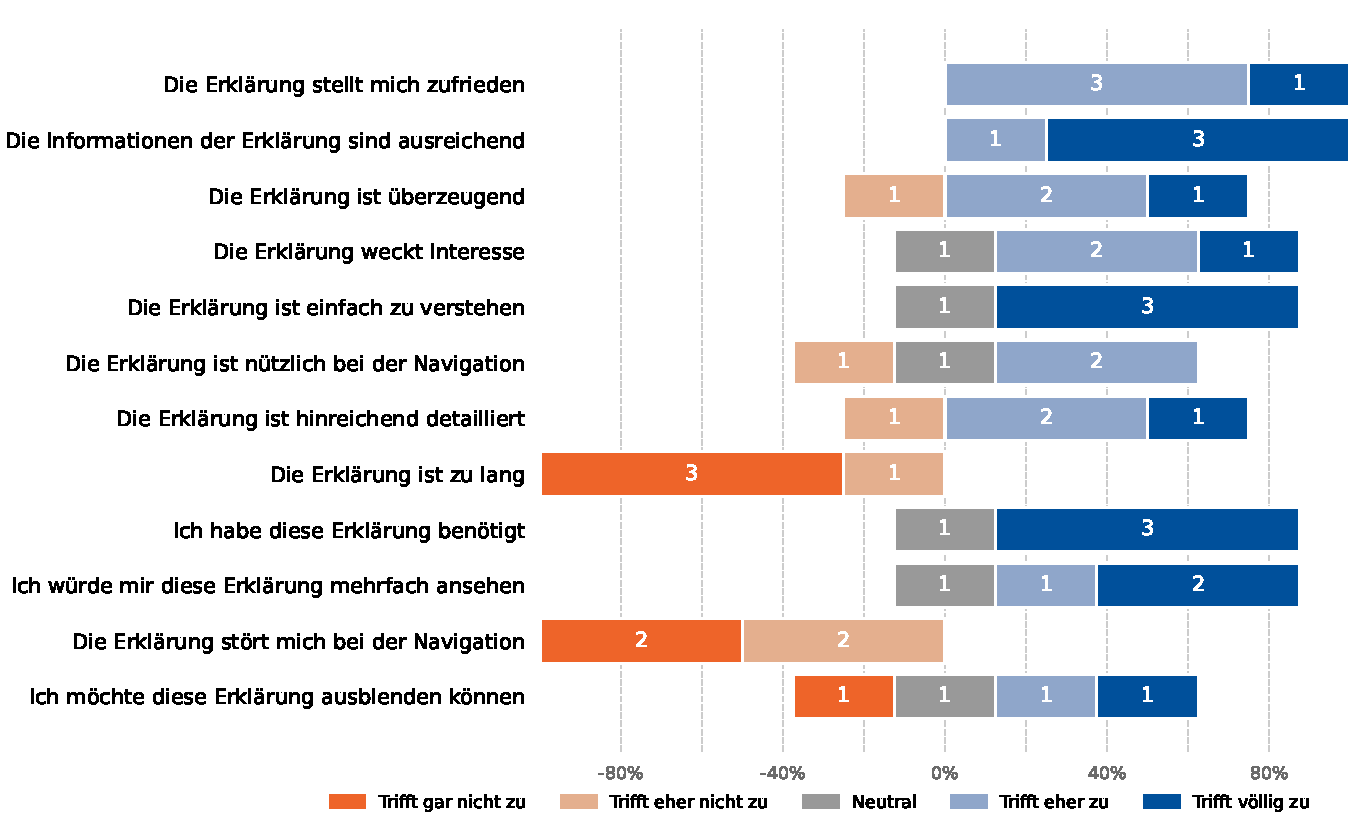
\includegraphics[width=\textwidth]{contents/06_model_evaluation/02_evaluation/res/qualitativeFeedback-01_collaborative_routing.pdf}
    \caption{Qualitative Erklärung 1}
    \label{fig:qualitative_evaluation_explanation1}
\end{figure}

\begin{figure}[htb!]
    \centering
    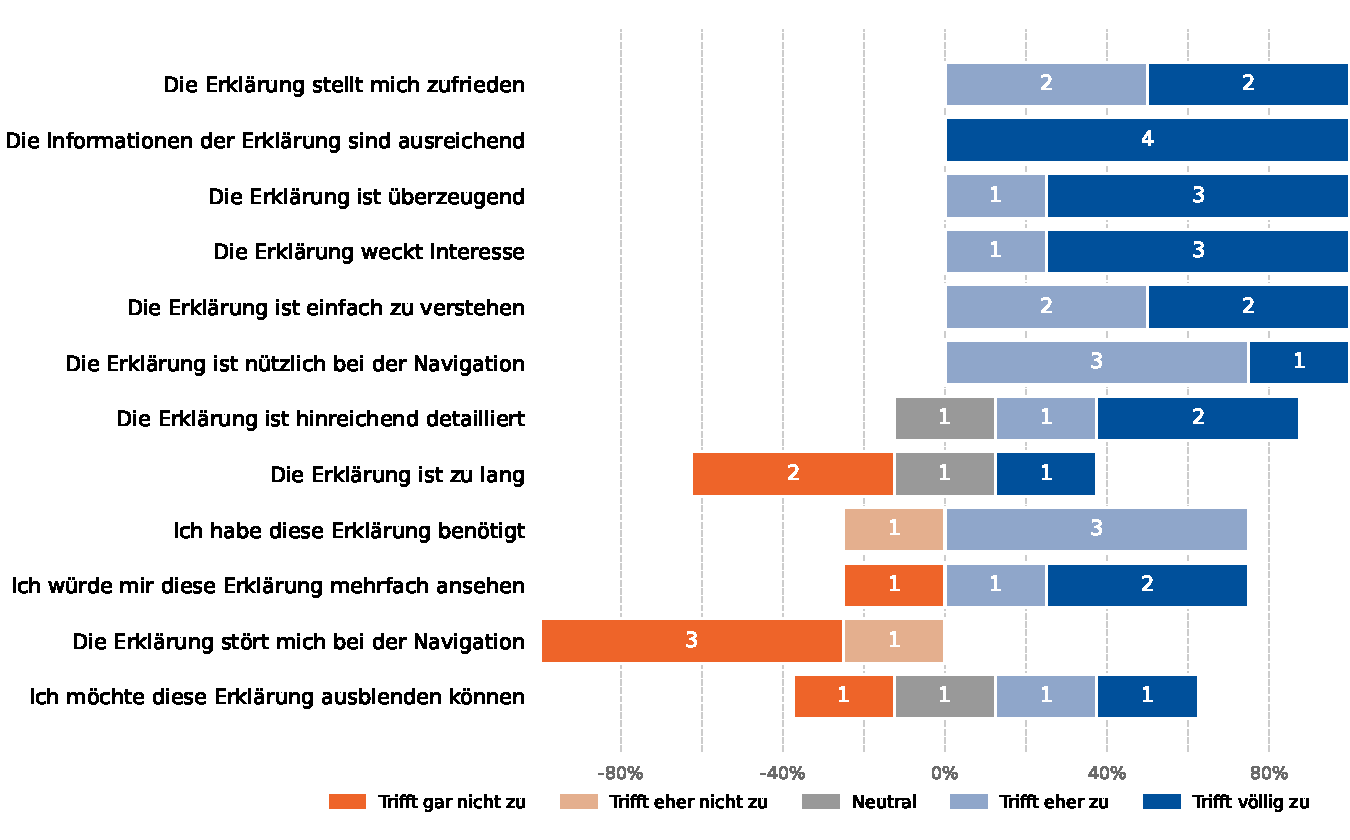
\includegraphics[width=\textwidth]{contents/06_model_evaluation/02_evaluation/res/qualitativeFeedback-02_collaborative_algorithm.pdf}
    \caption{Qualitative Erklärung 2}
    \label{fig:qualitative_evaluation_explanation2}
\end{figure}

\begin{figure}[htb!]
    \centering
    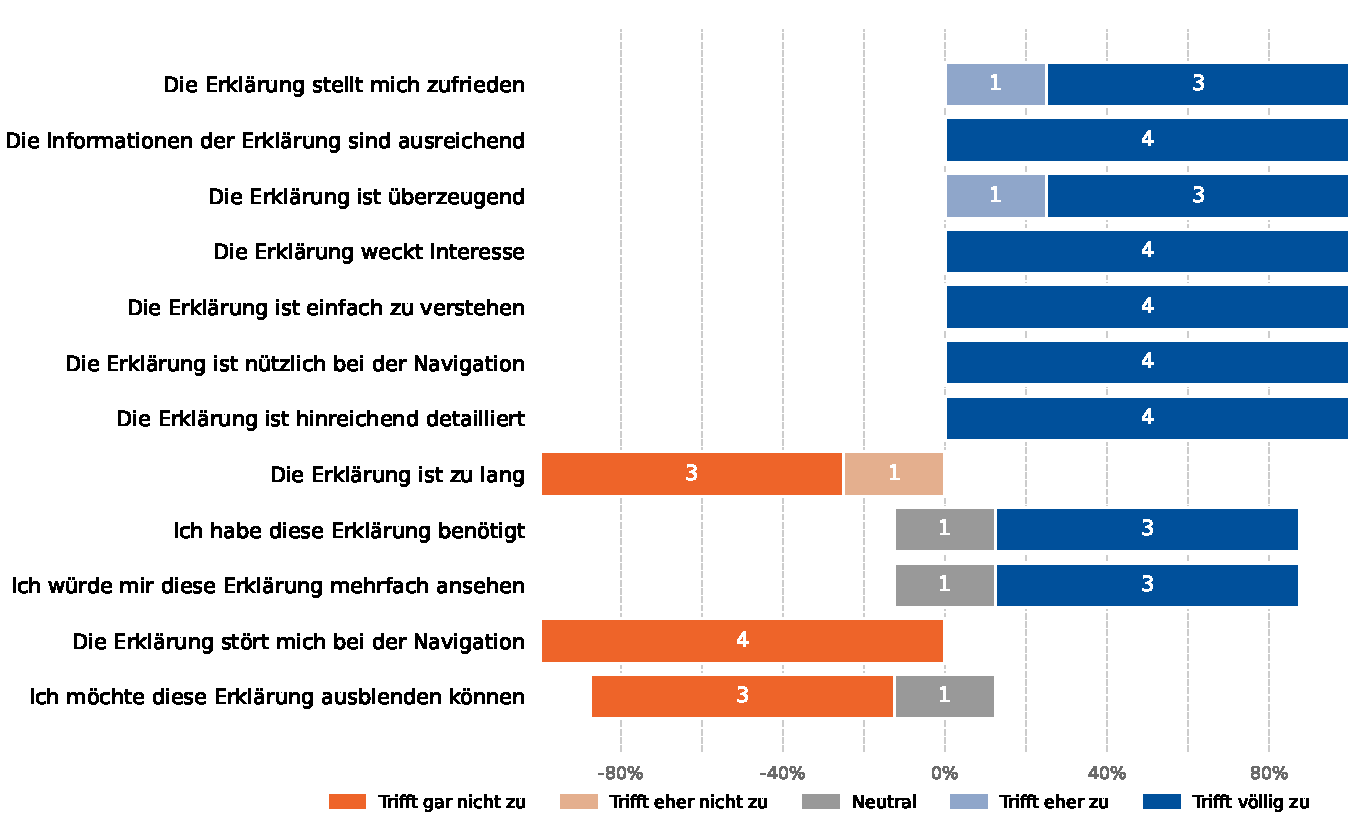
\includegraphics[width=\textwidth]{contents/06_model_evaluation/02_evaluation/res/qualitativeFeedback-03_traffic_volume.pdf}
    \caption{Qualitative Erklärung 3}
    \label{fig:qualitative_evaluation_explanation3}
\end{figure}

\begin{figure}[htb!]
    \centering
    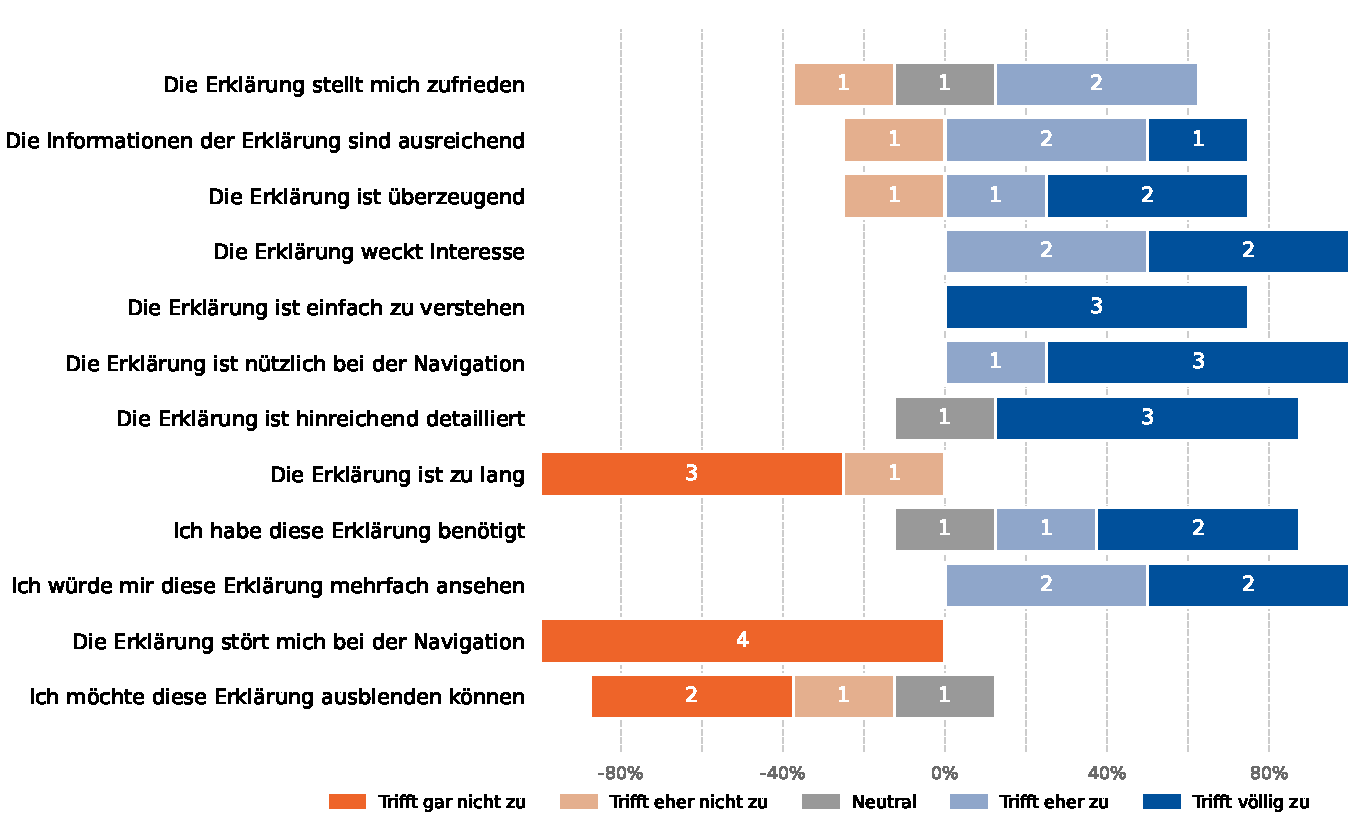
\includegraphics[width=\textwidth]{contents/06_model_evaluation/02_evaluation/res/qualitativeFeedback-04_position_accuracy.pdf}
    \caption{Qualitative Erklärung 4}
    \label{fig:qualitative_evaluation_explanation4}
\end{figure}